\documentclass[12pt]{standalone}

\usepackage{tikz}

\begin{document}
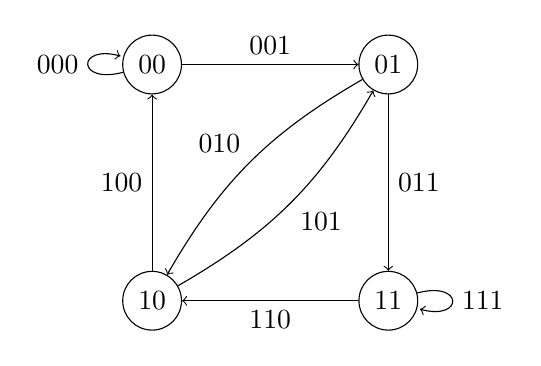
\begin{tikzpicture}[x=3cm,y=3cm]

\begin{scope}[every node/.style={circle,draw}]
    \node (0) at (0,1) {$00$};
    \node (1) at (1,1) {$01$};
    \node (2) at (0,0) {$10$};
    \node (3) at (1,0) {$11$};
\end{scope}

\path (0) edge[->,loop left] node[left] {$000$} ()
        edge [->] node[above] {$001$} (1)
    (1) edge [->,bend right=15] node[above left] {$010$} (2)
        edge [->] node[right] {$011$} (3)
    (2) edge [->] node[left] {$100$} (0)
        edge [->,bend right=15] node[below right] {$101$} (1)
    (3) edge [->] node[below] {$110$} (2)
        edge [->,loop right] node[right] {$111$} ();


\end{tikzpicture}
\end{document}
